\defi{5.0} Un \textbf{cuadrilátero} es una cuaterna ordenada de puntos [vértices] de $\P$, $(P, Q, R, S)$ formada por los segmentos $[P,Q], [Q,R], [R,S], [S,P]$ [lados] si dos cualesquiera segmentos son disjuntos o tienen un extremo en común. Dos vértices extremos del mismo lado son adyacentes y, si no, son opuestos.

\defi{5.1} Un cuadrilátero $\square PABC$ es un \textbf{paralelogramo} si $\m[P,B] = \m[A,C] = M$, donde los segmentos $[P,B]$ y $[A,C]$ son las diagonales, y $M$ es el centro.

\obs{5.2} Sea $\square PABC$ con centro $M$. Por las propiedades de las reflexiones centrales, se tiene que $\sigma_M(P) = B$ y $\sigma_M(A) = C$ [y viceversa]. Además, por tales propiedades, se tiene que $r_{PA} \parallel r_{BC}$ y $r_{PC} \parallel r_{AB}$; y $d(P,A) = d(B, C)$ y $d(P,C) = d(A,B)$. 

\obs{5.3} Si existen tres puntos $P,A,C$ no alineados, se puede construir un paralelogramo de varias maneras. Una forma es aplicar el axioma de las paralelas y proyectar $r_{PA}$ en $C$, y $r_{PC}$ en $A$. Otra forma es obtener $M  = \m[C,A]$, crear la recta $r_{PM}$ y proyectar el punto $B$ como el que $PM = d(P,M) = d(M,B) = MB$.

\tma{5.5 [Tales]} Sea $\triangle PAB$ y sean $A' \in [P,A]$, $B' \in  [P,B]$ dos puntos tales que $r_{AB} \parallel r_{A'B'}$. En estas condiciones se tiene que $\frac{PA'}{PA} = \frac{PB'}{PB}$.

\begin{figure}[H]
	\centering
	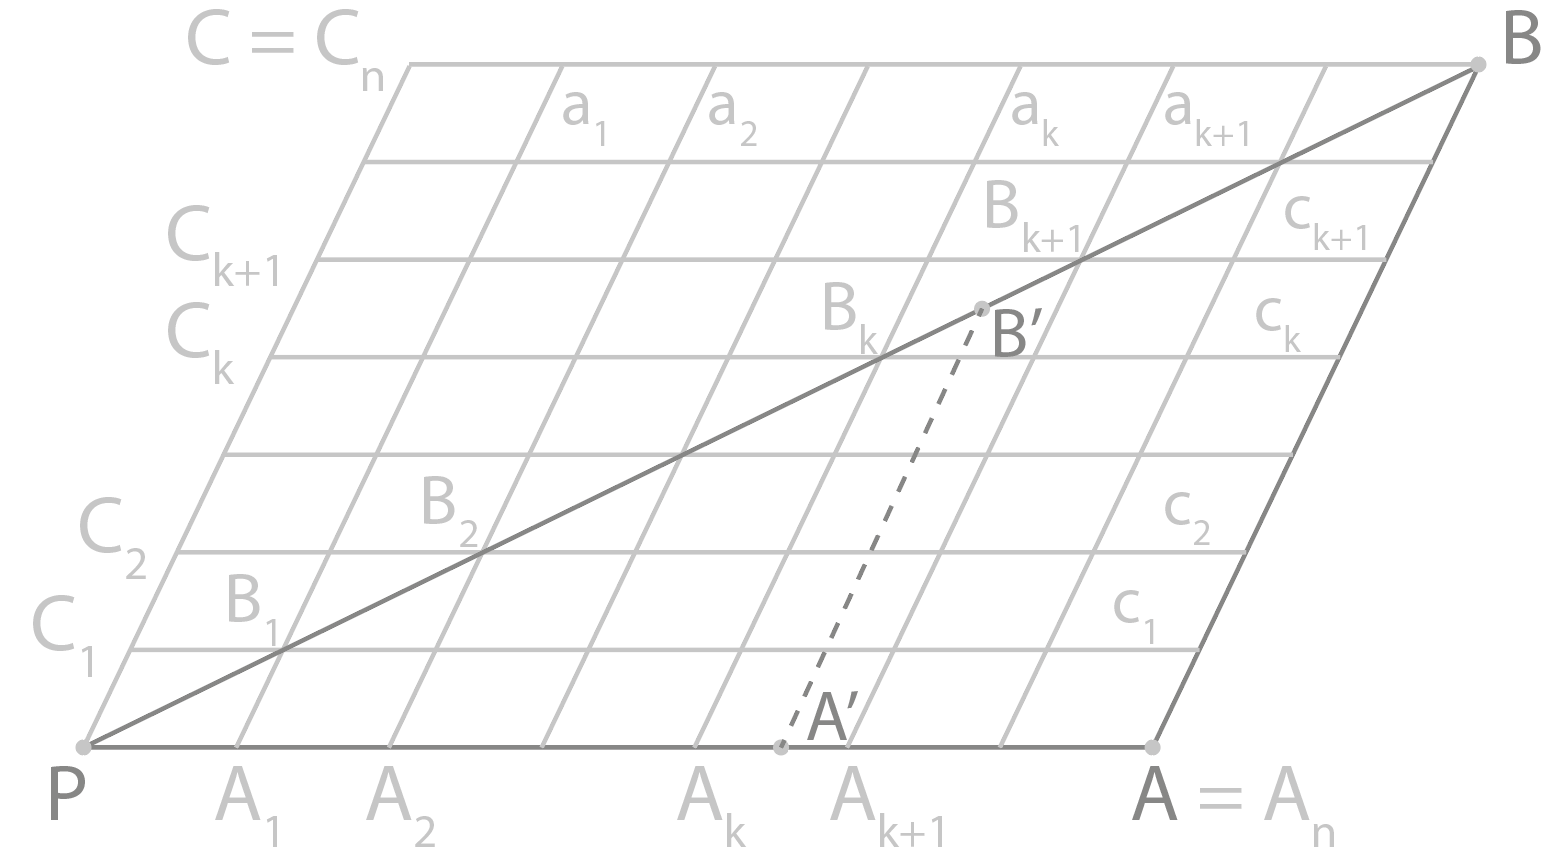
\includegraphics[width=8.2cm]{figuras/5-5.png}
	\vspace{-1em}
\end{figure}

\dem{Vamos a basar la demostración en la figura de arriba. 
Diseñamos el paralelogramo $\square PABC$ y dividimos el lado $[P,A]$ en $n$ segmentos con puntos de división $A_1, A_2, \cdots, A_n$, de modo que $d(A_i,A_{i+1}) = \frac{d(P,A)}{n}$. El mismo proceso se realiza con el lado $[P,C]$. Además, introducimos las rectas $a_k\parallel r_{PC}$ y $c_k\parallel r_{PA}$, de modo que el punto $P_{kl}$ es la intersección de $a_k$ con $c_l$. Vemos que $B_i = P_{ii}$. También observamos que existen los paralelogramos $\square A_kA_{k+1}P_{k+1,l}P_{k,l}$ y $\square C_lC_{l+1}P_{k,l+1}P_{k,l}$, de modo que $P_{kl}P_{k+1,l} = \frac{PA}{n}$ y $P_{kl}P_{k,l+1} = \frac{PC}{n}$.\linebreak
Ahora consideramos $B_k$. Sabemos que $\sigma_{B_k}(r) \parallel r$, $\sigma_{B_k}(c_k) = c_k$ y $\sigma_{B_k}(P_{k-1,k}) = P_{k+1,k}$. También, como $a_{k-1} \parallel a_{k+1}$, $\sigma_{B_k}(a_{k-1}) = a_{k+1}$, y por el mismo criterio, $\sigma_{B_k}(c_{k-1}) = c_{k+1}$. Con esto demostramos que $$\sigma_{B_k}(B_{k-1}) =\sigma_{B_k}(P_{k-1, k-1}) = P_{k+1, k+1}= B_{k+1}$$
Por tanto, los puntos $B_{k-1}, B_k, B_{k+1}$ están alineados y $B_{k-1}B_k = B_kB_{k+1}$. Por tanto, $B_kB_{k+1} = \frac{PB}{n}$.\linebreak
Es decir, hemos demostrado que
$$P_{kl}P_{k+1,l} = \frac{PA}{n} \quad  P_{kl}P_{k,l+1} = \frac{PC}{n} \quad P_{kl}P_{k+1,l+1} =  \frac{PB}{n}$$
Si reordenamos, tenemos que 
$$\frac{PA_k}{PA} = \frac{P_{0,0}P_{k,0}}{PA} = \frac{k}{n} = \frac{P_{0,0}P_{k,k}}{PB} =  \frac{PB_k}{PB}$$
Y con esto demostramos el teorema para los puntos $k$. Si tenemos $A'$ y $B'$ en la figura tales que $A' \in [A_k, A_{k+1}]$, de modo que $a' = r_{A'B'}$ está entre $a_k$ y $a_{k+1}$, y es paralelo a estas, haciendo que $B' \in [B_k, B_{k+1}]$. Por ser $A' \in [A_k, A_{k+1}]$ entonces $\frac{PA_k}{PA} \le \frac{PA'}{PA} \le \frac{PA_k}{PA}+\frac{1}{n}$ y, como $\frac{PA_k}{PA} = \frac{PB_k}{PB}$, entonces $\frac{PB_k}{PB} \le \frac{PA'}{PA} \le \frac{PB_k}{PB}+\frac{1}{n}$. Dado que $B'\in [B_k,B_{k+1}]$ entonces
$$\textcolor{SkyBlue}{\frac{PB'}{PB}-\frac{1}{n}} \le \frac{PB_k}{PB} \le \textcolor{SkyBlue}{\frac{PA'}{PA}} \le \frac{PB_k}{PB}+\frac{1}{n} \le \textcolor{SkyBlue}{\frac{PB'}{PB}+\frac{1}{n}}$$ 
Si nos fijamos en los elementos de azul, vemos que $n$ puede hacerse tan pequeño como queramos, de modo que, en el límite
$$\frac{PB'}{PB} \le \frac{PA'}{PA} \le \frac{PB'}{PB} \iff \frac{PB'}{PB} = \frac{PA'}{PA}$$ }

\cor{5.6} En base al teorema de Tales, se tiene que 
$$\frac{PA'}{PA} = \frac{PB'}{PB} = \frac{A'B'}{AB}$$

\defi{5.7} Dado un triángulo rectángulo $\triangle PAB$ con $\angle A$ recto, entonces la \textbf{hipotenusa} es el lado opuesto a $\angle A$, $[P,B]$. Los lados adyacentes, $[P,A],[B,A]$, son los \textbf{catetos}.
\begin{figure}[H]
	\centering
	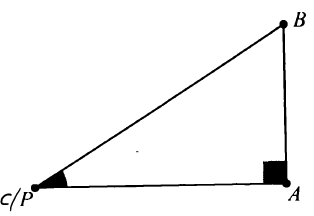
\includegraphics[width=3.5cm]{figuras/5-7.png}
	\vspace{-1em}
\end{figure}
\defi{5.8} Sea el triángulo rectángulo $\triangle PAB$ con $\angle A$ recto, entonces se definen las relaciones 
\begin{itemize}
	\item seno: $\text{sen}\angle P = \frac{BA}{PB}$
	\item coseno: $\text{cos}\angle P = \frac{PA}{PB}$
	\item tangente: $\text{tan}\angle P = \frac{BA}{PA}$
	\item cotangente: $\text{cot}\angle P = \frac{PA}{BA}$
\end{itemize}
\tma{5.10} Las razones trigonométricas para $\angle P$ no dependen del triángulo $\triangle PAB$, sólo de la clase de congruencia de $\angle P$.

\tma{5.12} Dado un triángulo rectángulo $\triangle ABC$ con $\angle A$ recto, la medida de los catetos, $AB,AC$, es menor que la de la hipotenusa $BC$.
\begin{figure}[H]
	\centering
	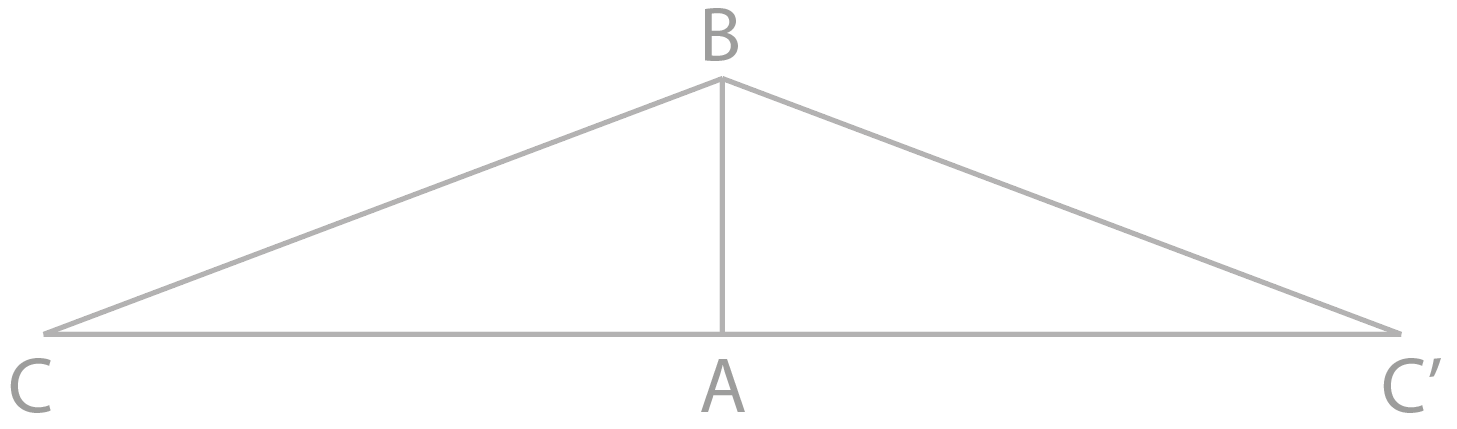
\includegraphics[width=6.5cm]{figuras/5-12.png}
	\vspace{-1em}
\end{figure}
\dem{Con la construcción anterior, vemos que los puntos $B, C, C'$ no están alineados, pues $C \in r_{AC}$ y $r_{AB}\perp r_{AC}$. Por la desigualdad triangular tenemos que $2AC = CC' < BC+BC' = 2BC$.}

\defi{5.13} La \textbf{medida de un ángulo} agudo $\angle P$ es el número real:
$$\measuredangle P = \arccos(\cos \angle P)$$
\tma{5.14 / 5.19} Si $\angle P = \angle Q$ entonces $\measuredangle P = \measuredangle Q$, sean $\angle P $ y $\angle Q$ agudos y obtusos.

\defi{5.15} Dado un ángulo $\angle{\overline{a}, \overline{b}_1} = \angle V$, un \textbf{ángulo suplementario} $\overline{\angle V} = \angle{\overline{a}, \overline{b}_2}$ es aquel donde $\overline{b}_1$ y $\overline{b}_2$ son las dos semirrectas de $b$ en $V$, y $\angle V$ y $\overline{\angle V}$ comparten $\overline{a}$. La suma de $\angle V$ y $\overline{\angle V}$ es un ángulo llano.

\tma{5.17} Si dos ángulos son congruentes, sus suplementarios lo son.

\defi{5.18} Para un ángulo obtuso $\angle P$ se tiene $\sen \angle P = \sen \overline{\angle P}$ y $\cos \angle P = -\cos \overline{\angle P}$

